\documentclass{standalone}
\usepackage{tikz}
\usetikzlibrary{patterns, positioning}


\begin{document}
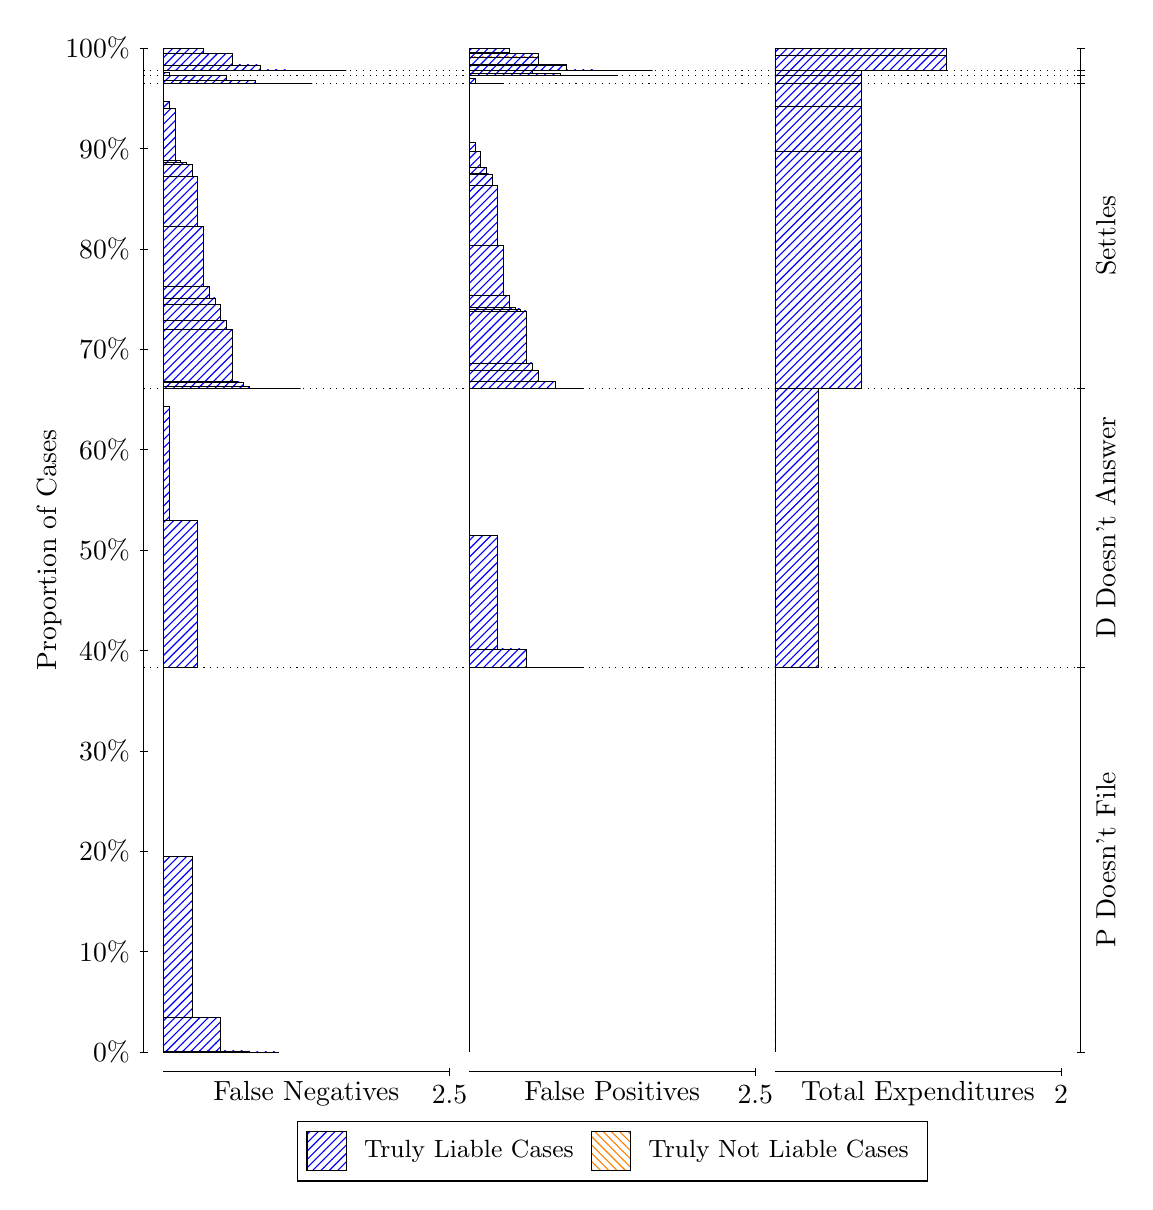
\begin{tikzpicture}
\draw[black, very thin] (1.5,1.75) -- (1.5,14.5);
\node[rotate=90, text=black, anchor=center] at (0.3, 8.125) {Proportion of Cases};
\draw[black, very thin] (1.45,1.75) -- (1.55,1.75);
\node[text=black, anchor=east] at (1.45, 1.75) {0\%};
\draw[black, very thin] (1.45,3.025) -- (1.55,3.025);
\node[text=black, anchor=east] at (1.45, 3.025) {10\%};
\draw[black, very thin] (1.45,4.3) -- (1.55,4.3);
\node[text=black, anchor=east] at (1.45, 4.3) {20\%};
\draw[black, very thin] (1.45,5.575) -- (1.55,5.575);
\node[text=black, anchor=east] at (1.45, 5.575) {30\%};
\draw[black, very thin] (1.45,6.85) -- (1.55,6.85);
\node[text=black, anchor=east] at (1.45, 6.85) {40\%};
\draw[black, very thin] (1.45,8.125) -- (1.55,8.125);
\node[text=black, anchor=east] at (1.45, 8.125) {50\%};
\draw[black, very thin] (1.45,9.4) -- (1.55,9.4);
\node[text=black, anchor=east] at (1.45, 9.4) {60\%};
\draw[black, very thin] (1.45,10.675) -- (1.55,10.675);
\node[text=black, anchor=east] at (1.45, 10.675) {70\%};
\draw[black, very thin] (1.45,11.95) -- (1.55,11.95);
\node[text=black, anchor=east] at (1.45, 11.95) {80\%};
\draw[black, very thin] (1.45,13.225) -- (1.55,13.225);
\node[text=black, anchor=east] at (1.45, 13.225) {90\%};
\draw[black, very thin] (1.45,14.5) -- (1.55,14.5);
\node[text=black, anchor=east] at (1.45, 14.5) {100\%};

\draw[black, very thin] (13.4,1.75) -- (13.4,14.5);
\draw[black, very thin] (13.35,1.75) -- (13.45,1.75);
\node[anchor=west] at (13.35, 1.75) {};
\draw[black, very thin] (13.35,6.6349) -- (13.45,6.6349);
\node[anchor=west] at (13.35, 6.6349) {};
\draw[black, very thin] (13.35,10.181) -- (13.45,10.181);
\node[anchor=west] at (13.35, 10.181) {};
\draw[black, very thin] (13.35,14.05) -- (13.45,14.05);
\node[anchor=west] at (13.35, 14.05) {};
\draw[black, very thin] (13.35,14.152) -- (13.45,14.152);
\node[anchor=west] at (13.35, 14.152) {};
\draw[black, very thin] (13.35,14.217) -- (13.45,14.217);
\node[anchor=west] at (13.35, 14.217) {};
\draw[black, very thin] (13.35,14.5) -- (13.45,14.5);
\node[anchor=west] at (13.35, 14.5) {};

\draw[black, very thin, pattern color=blue, pattern=north east lines] (1.75,1.75) rectangle (3.2033,1.7501);
\draw[black, very thin, pattern color=blue, pattern=north east lines] (1.75,1.7501) rectangle (2.84,1.7643);
\draw[black, very thin, pattern color=blue, pattern=north east lines] (1.75,1.7643) rectangle (2.4767,2.1937);
\draw[black, very thin, pattern color=blue, pattern=north east lines] (1.75,2.1937) rectangle (2.1133,4.2303);
\draw[black, very thin, pattern color=orange, pattern=north west lines] (1.75,4.2303) rectangle (1.75,4.2303);
\draw[black, very thin, pattern color=blue, pattern=north east lines] (1.75,4.2303) rectangle (1.75,6.6349);
\draw[black, very thin, pattern color=blue, pattern=north east lines] (1.75,6.6349) rectangle (2.186,8.5048);
\draw[black, very thin, pattern color=blue, pattern=north east lines] (1.75,8.5048) rectangle (1.8227,9.9457);
\draw[black, very thin, pattern color=orange, pattern=north west lines] (1.75,9.9457) rectangle (1.75,9.9457);
\draw[black, very thin, pattern color=blue, pattern=north east lines] (1.75,9.9457) rectangle (1.75,10.181);
\draw[black, very thin, pattern color=blue, pattern=north east lines] (1.75,10.181) rectangle (3.494,10.181);
\draw[black, very thin, pattern color=blue, pattern=north east lines] (1.75,10.181) rectangle (3.2033,10.181);
\draw[black, very thin, pattern color=blue, pattern=north east lines] (1.75,10.181) rectangle (3.1307,10.182);
\draw[black, very thin, pattern color=blue, pattern=north east lines] (1.75,10.182) rectangle (3.058,10.182);
\draw[black, very thin, pattern color=blue, pattern=north east lines] (1.75,10.182) rectangle (2.9127,10.182);
\draw[black, very thin, pattern color=blue, pattern=north east lines] (1.75,10.182) rectangle (2.84,10.21);
\draw[black, very thin, pattern color=blue, pattern=north east lines] (1.75,10.21) rectangle (2.7673,10.259);
\draw[black, very thin, pattern color=blue, pattern=north east lines] (1.75,10.259) rectangle (2.6947,10.266);
\draw[black, very thin, pattern color=blue, pattern=north east lines] (1.75,10.266) rectangle (2.622,10.926);
\draw[black, very thin, pattern color=blue, pattern=north east lines] (1.75,10.926) rectangle (2.5493,11.041);
\draw[black, very thin, pattern color=blue, pattern=north east lines] (1.75,11.041) rectangle (2.4767,11.245);
\draw[black, very thin, pattern color=blue, pattern=north east lines] (1.75,11.245) rectangle (2.404,11.318);
\draw[black, very thin, pattern color=blue, pattern=north east lines] (1.75,11.318) rectangle (2.404,11.328);
\draw[black, very thin, pattern color=blue, pattern=north east lines] (1.75,11.328) rectangle (2.3313,11.476);
\draw[black, very thin, pattern color=blue, pattern=north east lines] (1.75,11.476) rectangle (2.2587,12.236);
\draw[black, very thin, pattern color=blue, pattern=north east lines] (1.75,12.236) rectangle (2.186,12.869);
\draw[black, very thin, pattern color=blue, pattern=north east lines] (1.75,12.869) rectangle (2.1133,13.025);
\draw[black, very thin, pattern color=blue, pattern=north east lines] (1.75,13.025) rectangle (2.0407,13.043);
\draw[black, very thin, pattern color=blue, pattern=north east lines] (1.75,13.043) rectangle (2.0407,13.043);
\draw[black, very thin, pattern color=blue, pattern=north east lines] (1.75,13.043) rectangle (1.968,13.069);
\draw[black, very thin, pattern color=blue, pattern=north east lines] (1.75,13.069) rectangle (1.8953,13.73);
\draw[black, very thin, pattern color=blue, pattern=north east lines] (1.75,13.73) rectangle (1.8227,13.826);
\draw[black, very thin, pattern color=orange, pattern=north west lines] (1.75,13.826) rectangle (1.75,13.826);
\draw[black, very thin, pattern color=blue, pattern=north east lines] (1.75,13.826) rectangle (1.75,14.05);
\draw[black, very thin, pattern color=blue, pattern=north east lines] (1.75,14.05) rectangle (3.6393,14.05);
\draw[black, very thin, pattern color=blue, pattern=north east lines] (1.75,14.05) rectangle (3.276,14.05);
\draw[black, very thin, pattern color=blue, pattern=north east lines] (1.75,14.05) rectangle (2.9127,14.088);
\draw[black, very thin, pattern color=blue, pattern=north east lines] (1.75,14.088) rectangle (2.5493,14.15);
\draw[black, very thin, pattern color=blue, pattern=north east lines] (1.75,14.15) rectangle (2.186,14.152);
\draw[black, very thin, pattern color=orange, pattern=north west lines] (1.75,14.152) rectangle (1.75,14.152);
\draw[black, very thin, pattern color=blue, pattern=north east lines] (1.75,14.152) rectangle (2.186,14.152);
\draw[black, very thin, pattern color=blue, pattern=north east lines] (1.75,14.152) rectangle (1.8227,14.193);
\draw[black, very thin, pattern color=orange, pattern=north west lines] (1.75,14.193) rectangle (1.75,14.193);
\draw[black, very thin, pattern color=blue, pattern=north east lines] (1.75,14.193) rectangle (1.75,14.217);
\draw[black, very thin, pattern color=blue, pattern=north east lines] (1.75,14.217) rectangle (4.0753,14.217);
\draw[black, very thin, pattern color=blue, pattern=north east lines] (1.75,14.217) rectangle (3.712,14.217);
\draw[black, very thin, pattern color=blue, pattern=north east lines] (1.75,14.217) rectangle (3.3487,14.222);
\draw[black, very thin, pattern color=blue, pattern=north east lines] (1.75,14.222) rectangle (2.9853,14.287);
\draw[black, very thin, pattern color=blue, pattern=north east lines] (1.75,14.287) rectangle (2.622,14.43);
\draw[black, very thin, pattern color=blue, pattern=north east lines] (1.75,14.43) rectangle (2.2587,14.495);
\draw[black, very thin, pattern color=blue, pattern=north east lines] (1.75,14.495) rectangle (1.8953,14.5);
\draw[black, very thin, pattern color=orange, pattern=north west lines] (1.75,14.5) rectangle (1.75,14.5);
\draw[black, very thin, pattern color=blue, pattern=north east lines] (1.75,14.5) rectangle (1.75,14.5);
\draw[black, very thin, pattern color=orange, pattern=north west lines] (5.6333,1.75) rectangle (5.6333,1.75);
\draw[black, very thin, pattern color=blue, pattern=north east lines] (5.6333,1.75) rectangle (5.6333,6.6349);
\draw[black, very thin, pattern color=orange, pattern=north west lines] (5.6333,6.6349) rectangle (7.0867,6.6349);
\draw[black, very thin, pattern color=blue, pattern=north east lines] (5.6333,6.6349) rectangle (7.0867,6.6349);
\draw[black, very thin, pattern color=blue, pattern=north east lines] (5.6333,6.6349) rectangle (6.7233,6.6359);
\draw[black, very thin, pattern color=blue, pattern=north east lines] (5.6333,6.6359) rectangle (6.36,6.8701);
\draw[black, very thin, pattern color=blue, pattern=north east lines] (5.6333,6.8701) rectangle (5.9967,8.3109);
\draw[black, very thin, pattern color=blue, pattern=north east lines] (5.6333,8.3109) rectangle (5.6333,10.181);
\draw[black, very thin, pattern color=orange, pattern=north west lines] (5.6333,10.181) rectangle (7.0867,10.181);
\draw[black, very thin, pattern color=blue, pattern=north east lines] (5.6333,10.181) rectangle (7.0867,10.181);
\draw[black, very thin, pattern color=orange, pattern=north west lines] (5.6333,10.181) rectangle (6.9413,10.181);
\draw[black, very thin, pattern color=blue, pattern=north east lines] (5.6333,10.181) rectangle (6.9413,10.181);
\draw[black, very thin, pattern color=orange, pattern=north west lines] (5.6333,10.181) rectangle (6.796,10.181);
\draw[black, very thin, pattern color=blue, pattern=north east lines] (5.6333,10.181) rectangle (6.796,10.181);
\draw[black, very thin, pattern color=blue, pattern=north east lines] (5.6333,10.181) rectangle (6.7233,10.263);
\draw[black, very thin, pattern color=orange, pattern=north west lines] (5.6333,10.263) rectangle (6.6507,10.263);
\draw[black, very thin, pattern color=blue, pattern=north east lines] (5.6333,10.263) rectangle (6.6507,10.264);
\draw[black, very thin, pattern color=blue, pattern=north east lines] (5.6333,10.264) rectangle (6.578,10.264);
\draw[black, very thin, pattern color=orange, pattern=north west lines] (5.6333,10.264) rectangle (6.5053,10.264);
\draw[black, very thin, pattern color=blue, pattern=north east lines] (5.6333,10.264) rectangle (6.5053,10.405);
\draw[black, very thin, pattern color=blue, pattern=north east lines] (5.6333,10.405) rectangle (6.4327,10.501);
\draw[black, very thin, pattern color=blue, pattern=north east lines] (5.6333,10.501) rectangle (6.36,11.162);
\draw[black, very thin, pattern color=blue, pattern=north east lines] (5.6333,11.162) rectangle (6.2873,11.188);
\draw[black, very thin, pattern color=orange, pattern=north west lines] (5.6333,11.188) rectangle (6.2147,11.188);
\draw[black, very thin, pattern color=blue, pattern=north east lines] (5.6333,11.188) rectangle (6.2147,11.188);
\draw[black, very thin, pattern color=blue, pattern=north east lines] (5.6333,11.188) rectangle (6.2147,11.206);
\draw[black, very thin, pattern color=blue, pattern=north east lines] (5.6333,11.206) rectangle (6.142,11.362);
\draw[black, very thin, pattern color=blue, pattern=north east lines] (5.6333,11.362) rectangle (6.0693,11.995);
\draw[black, very thin, pattern color=blue, pattern=north east lines] (5.6333,11.995) rectangle (5.9967,12.755);
\draw[black, very thin, pattern color=blue, pattern=north east lines] (5.6333,12.755) rectangle (5.924,12.903);
\draw[black, very thin, pattern color=blue, pattern=north east lines] (5.6333,12.903) rectangle (5.8513,12.914);
\draw[black, very thin, pattern color=blue, pattern=north east lines] (5.6333,12.914) rectangle (5.8513,12.986);
\draw[black, very thin, pattern color=blue, pattern=north east lines] (5.6333,12.986) rectangle (5.7787,13.19);
\draw[black, very thin, pattern color=blue, pattern=north east lines] (5.6333,13.19) rectangle (5.706,13.305);
\draw[black, very thin, pattern color=blue, pattern=north east lines] (5.6333,13.305) rectangle (5.6333,14.05);
\draw[black, very thin, pattern color=orange, pattern=north west lines] (5.6333,14.05) rectangle (6.0693,14.05);
\draw[black, very thin, pattern color=blue, pattern=north east lines] (5.6333,14.05) rectangle (6.0693,14.052);
\draw[black, very thin, pattern color=blue, pattern=north east lines] (5.6333,14.052) rectangle (5.706,14.114);
\draw[black, very thin, pattern color=blue, pattern=north east lines] (5.6333,14.114) rectangle (5.6333,14.152);
\draw[black, very thin, pattern color=orange, pattern=north west lines] (5.6333,14.152) rectangle (7.5227,14.152);
\draw[black, very thin, pattern color=blue, pattern=north east lines] (5.6333,14.152) rectangle (7.5227,14.152);
\draw[black, very thin, pattern color=blue, pattern=north east lines] (5.6333,14.152) rectangle (7.1593,14.152);
\draw[black, very thin, pattern color=blue, pattern=north east lines] (5.6333,14.152) rectangle (6.796,14.176);
\draw[black, very thin, pattern color=blue, pattern=north east lines] (5.6333,14.176) rectangle (6.4327,14.216);
\draw[black, very thin, pattern color=blue, pattern=north east lines] (5.6333,14.216) rectangle (6.0693,14.217);
\draw[black, very thin, pattern color=orange, pattern=north west lines] (5.6333,14.217) rectangle (7.9587,14.217);
\draw[black, very thin, pattern color=blue, pattern=north east lines] (5.6333,14.217) rectangle (7.9587,14.217);
\draw[black, very thin, pattern color=orange, pattern=north west lines] (5.6333,14.217) rectangle (7.5953,14.217);
\draw[black, very thin, pattern color=blue, pattern=north east lines] (5.6333,14.217) rectangle (7.5953,14.217);
\draw[black, very thin, pattern color=orange, pattern=north west lines] (5.6333,14.217) rectangle (7.232,14.217);
\draw[black, very thin, pattern color=blue, pattern=north east lines] (5.6333,14.217) rectangle (7.232,14.222);
\draw[black, very thin, pattern color=blue, pattern=north east lines] (5.6333,14.222) rectangle (6.8687,14.287);
\draw[black, very thin, pattern color=orange, pattern=north west lines] (5.6333,14.287) rectangle (6.8687,14.287);
\draw[black, very thin, pattern color=blue, pattern=north east lines] (5.6333,14.287) rectangle (6.8687,14.288);
\draw[black, very thin, pattern color=blue, pattern=north east lines] (5.6333,14.288) rectangle (6.5053,14.388);
\draw[black, very thin, pattern color=orange, pattern=north west lines] (5.6333,14.388) rectangle (6.5053,14.388);
\draw[black, very thin, pattern color=blue, pattern=north east lines] (5.6333,14.388) rectangle (6.5053,14.43);
\draw[black, very thin, pattern color=blue, pattern=north east lines] (5.6333,14.43) rectangle (6.142,14.447);
\draw[black, very thin, pattern color=blue, pattern=north east lines] (5.6333,14.447) rectangle (6.142,14.495);
\draw[black, very thin, pattern color=blue, pattern=north east lines] (5.6333,14.495) rectangle (5.7787,14.495);
\draw[black, very thin, pattern color=blue, pattern=north east lines] (5.6333,14.495) rectangle (5.7787,14.5);
\draw[black, very thin, pattern color=blue, pattern=north east lines] (5.6333,14.5) rectangle (5.6333,14.5);
\draw[black, very thin, pattern color=orange, pattern=north west lines] (9.5167,1.75) rectangle (9.5167,1.75);
\draw[black, very thin, pattern color=blue, pattern=north east lines] (9.5167,1.75) rectangle (9.5167,6.6349);
\draw[black, very thin, pattern color=orange, pattern=north west lines] (9.5167,6.6349) rectangle (10.062,6.6349);
\draw[black, very thin, pattern color=blue, pattern=north east lines] (9.5167,6.6349) rectangle (10.062,10.181);
\draw[black, very thin, pattern color=orange, pattern=north west lines] (9.5167,10.181) rectangle (10.607,10.181);
\draw[black, very thin, pattern color=blue, pattern=north east lines] (9.5167,10.181) rectangle (10.607,13.189);
\draw[black, very thin, pattern color=orange, pattern=north west lines] (9.5167,13.189) rectangle (10.607,13.189);
\draw[black, very thin, pattern color=blue, pattern=north east lines] (9.5167,13.189) rectangle (10.607,13.762);
\draw[black, very thin, pattern color=orange, pattern=north west lines] (9.5167,13.762) rectangle (10.607,13.762);
\draw[black, very thin, pattern color=blue, pattern=north east lines] (9.5167,13.762) rectangle (10.607,14.05);
\draw[black, very thin, pattern color=orange, pattern=north west lines] (9.5167,14.05) rectangle (10.607,14.05);
\draw[black, very thin, pattern color=blue, pattern=north east lines] (9.5167,14.05) rectangle (10.607,14.152);
\draw[black, very thin, pattern color=orange, pattern=north west lines] (9.5167,14.152) rectangle (10.607,14.152);
\draw[black, very thin, pattern color=blue, pattern=north east lines] (9.5167,14.152) rectangle (10.607,14.217);
\draw[black, very thin, pattern color=orange, pattern=north west lines] (9.5167,14.217) rectangle (11.697,14.217);
\draw[black, very thin, pattern color=blue, pattern=north east lines] (9.5167,14.217) rectangle (11.697,14.405);
\draw[black, very thin, pattern color=orange, pattern=north west lines] (9.5167,14.405) rectangle (11.697,14.405);
\draw[black, very thin, pattern color=blue, pattern=north east lines] (9.5167,14.405) rectangle (11.697,14.5);
\draw[black, dotted] (1.5,6.6349) -- (13.4,6.6349);
\draw[black, dotted] (1.5,10.181) -- (13.4,10.181);
\draw[black, dotted] (1.5,14.05) -- (13.4,14.05);
\draw[black, dotted] (1.5,14.152) -- (13.4,14.152);
\draw[black, dotted] (1.5,14.217) -- (13.4,14.217);
\draw[black, very thin] (1.75,1.5) -- (5.3833,1.5);
\node[text=black, anchor=north] at (3.5667, 1.5) {False Negatives};
\draw[black, very thin] (5.3833,1.45) -- (5.3833,1.55);
\node[text=black, anchor=north] at (5.3833, 1.45) {2.5};

\draw[black, very thin] (5.6333,1.5) -- (9.2667,1.5);
\node[text=black, anchor=north] at (7.45, 1.5) {False Positives};
\draw[black, very thin] (9.2667,1.45) -- (9.2667,1.55);
\node[text=black, anchor=north] at (9.2667, 1.45) {2.5};

\draw[black, very thin] (9.5167,1.5) -- (13.15,1.5);
\node[text=black, anchor=north] at (11.333, 1.5) {Total Expenditures};
\draw[black, very thin] (13.15,1.45) -- (13.15,1.55);
\node[text=black, anchor=north] at (13.15, 1.45) {2};

\node[text=black, centered, rotate=90] at (13.72, 4.1924) {P Doesn't File};
\node[text=black, centered, rotate=90] at (13.72, 8.4079) {D Doesn't Answer};
\node[text=black, centered, rotate=90] at (13.72, 12.116) {Settles};




\draw (7.449999999999999,1.5) node[draw=none] (baseCoordinate) {};
\begin{scope}[align=center]
        \matrix[scale=0.5, draw=black, below=0.5cm of baseCoordinate, nodes={draw}, column sep=0.1cm]{
            \node[rectangle, draw, minimum width=0.5cm, minimum height=0.5cm, pattern color=blue, pattern=north east lines] {}; &
            \node[draw=none, font=\small, text=black] (B) {Truly Liable Cases}; &
            \node[rectangle, draw, minimum width=0.5cm, minimum height=0.5cm, pattern color=orange, pattern=north west lines] {}; &
            \node[draw=none, font=\small, text=black] (B) {Truly Not Liable Cases}; \\
            };
\end{scope}

\end{tikzpicture}
\end{document}